\documentclass{article}
\usepackage[margin=2cm]{geometry}
\usepackage{float}
\usepackage{graphicx}

% Import custom listings colourings.
\usepackage{listings}
\usepackage{color}
\usepackage{xcolor}

%listings grey title/caption box 
\usepackage{caption}
\DeclareCaptionFont{white}{\color{white}}
\DeclareCaptionFormat{listing}{\colorbox{gray}{\parbox{\textwidth}{#1#2#3}}}
\captionsetup[lstlisting]{format=listing,labelfont=white,textfont=white}

% Java custom colours
\definecolor{javared}{rgb}{0.6,0,0} % for strings
\definecolor{javagreen}{rgb}{0.25,0.5,0.35} % comments
\definecolor{javapurple}{rgb}{0.5,0,0.35} % keywords
\definecolor{javadocblue}{rgb}{0.25,0.35,0.75} % javadoc

%Java custom config
\lstdefinestyle{customjava}{language=java,
basicstyle=\footnotesize,
keywordstyle=\color{javapurple}\bfseries,
stringstyle=\color{javared},
commentstyle=\color{javagreen},
morecomment=[s][\color{javadocblue}]{/**}{*/},
numbers=left,
numberstyle=\tiny\color{black},
stepnumber=1,
numbersep=10pt,
tabsize=4,
showspaces=false,
showstringspaces=false
}

%C++ custom colours
\definecolor{Brown}{cmyk}{0,0.81,1,0.60}
\definecolor{OliveGreen}{cmyk}{0.64,0,0.95,0.40}
\definecolor{CadetBlue}{cmyk}{0.62,0.57,0.23,0}

%C++ custom config
\lstdefinestyle{customcpp}{language=c++,
basicstyle=\footnotesize,
keywordstyle=\color{OliveGreen}\bfseries,
stringstyle=\color{javared},
commentstyle=\color{CadetBlue},
morecomment=[s][\color{javadocblue}]{/**}{*/},
numbers=left,
numberstyle=\tiny\color{black},
stepnumber=1,
numbersep=10pt,
tabsize=4,
showspaces=false,
showstringspaces=false}

\lstset{showspaces=false, showstringspaces=false,    basicstyle=\footnotesize, columns=fullflexible} 

% Paragraph settings
\setlength{\parskip}{10pt plus 1pt minus 1pt
\setlength{\parindent}{0cm}}

\begin{document}
\title{CS22510 - Assignment 1 \\ Runners and Riders - "Out and About"}
\author{Samuel Jackson \\ \texttt{slj11@aber.ac.uk}}
\date{\today}
\maketitle

\section{Event Creation Program Documentation}

\subsection{Code Listing}
The following section provides the full code listing for the event creation program. This application is written using C++. Doxygen documentation is available via the provided CD.

\lstinputlisting[style=customcpp, language=c++, caption={eventcreator.h}]{"../Event Creator/eventcreator.h"}
\lstinputlisting[style=customcpp, language=c++, caption={eventcreator.cpp}]{"../Event Creator/eventcreator.cpp"}

\lstinputlisting[style=customcpp, language=c++, caption={event.h}]{"../Event Creator/event.h"}
\lstinputlisting[style=customcpp, language=c++, caption={event.cpp}]{"../Event Creator/event.cpp"}

\lstinputlisting[style=customcpp, language=c++, caption={entrant.h}]{"../Event Creator/entrant.h"}
\lstinputlisting[style=customcpp, language=c++, caption={entrant.cpp}]{"../Event Creator/entrant.cpp"}

\lstinputlisting[style=customcpp, language=c++, caption={course.h}]{"../Event Creator/course.h"}
\lstinputlisting[style=customcpp, language=c++, caption={course.cpp}]{"../Event Creator/course.cpp"}

\lstinputlisting[style=customcpp, language=c++, caption={fileio.h}]{"../Event Creator/fileio.h"}
\lstinputlisting[style=customcpp, language=c++, caption={fileio.cpp}]{"../Event Creator/fileio.cpp"}

\lstinputlisting[style=customcpp, language=c++, caption={ioscanner.h}]{"../Event Creator/ioscanner.h"}
\lstinputlisting[style=customcpp, language=c++, caption={ioscanner.cpp}]{"../Event Creator/ioscanner.cpp"}


\subsection{Compilation Output}
The following section shows the build log generated by Eclipse when compiling the Event Creation program.

\begin{center}
	\begin{lstlisting}[showstringspaces=false, caption={Build log of the C++ Event Creation Program}]
	
12:22:50 **** Build of configuration Debug for project Event Creator ****
make all 
Building file: ../course.cpp
Invoking: GCC C++ Compiler
g++ -O0 -g3 -Wall -c -fmessage-length=0 -MMD -MP -MF"course.d" -MT"course.d" -o "course.o" "../course.cpp"
Finished building: ../course.cpp
 
Building file: ../entrant.cpp
Invoking: GCC C++ Compiler
g++ -O0 -g3 -Wall -c -fmessage-length=0 -MMD -MP -MF"entrant.d" -MT"entrant.d" -o "entrant.o" "../entrant.cpp"
Finished building: ../entrant.cpp
 
Building file: ../event.cpp
Invoking: GCC C++ Compiler
g++ -O0 -g3 -Wall -c -fmessage-length=0 -MMD -MP -MF"event.d" -MT"event.d" -o "event.o" "../event.cpp"
Finished building: ../event.cpp
 
Building file: ../eventcreator.cpp
Invoking: GCC C++ Compiler
g++ -O0 -g3 -Wall -c -fmessage-length=0 -MMD -MP -MF"eventcreator.d" -MT"eventcreator.d" 
-o "eventcreator.o" "../eventcreator.cpp"
../eventcreator.cpp: In member function ‘int EventCreator::ChooseEvent()’:
../eventcreator.cpp:160:51: warning: comparison between signed and unsigned integer expressions [-Wsign-compare]
../eventcreator.cpp: In member function ‘char EventCreator::ChooseCourse(Event)’:
../eventcreator.cpp:194:52: warning: comparison between signed and unsigned integer expressions [-Wsign-compare]
Finished building: ../eventcreator.cpp
 
Building file: ../fileio.cpp
Invoking: GCC C++ Compiler
g++ -O0 -g3 -Wall -c -fmessage-length=0 -MMD -MP -MF"fileio.d" -MT"fileio.d" -o "fileio.o" "../fileio.cpp"
Finished building: ../fileio.cpp
 
Building file: ../ioscanner.cpp
Invoking: GCC C++ Compiler
g++ -O0 -g3 -Wall -c -fmessage-length=0 -MMD -MP -MF"ioscanner.d" -MT"ioscanner.d" -o "ioscanner.o" "../ioscanner.cpp"
../ioscanner.cpp: In member function ‘std::string IOScanner::ReadString(int)’:
../ioscanner.cpp:49:25: warning: comparison between signed and unsigned integer expressions [-Wsign-compare]
../ioscanner.cpp:52:29: warning: comparison between signed and unsigned integer expressions [-Wsign-compare]
Finished building: ../ioscanner.cpp
 
Building target: Event Creator
Invoking: GCC C++ Linker
g++  -o "Event Creator"  ./course.o ./entrant.o ./event.o ./eventcreator.o ./fileio.o ./ioscanner.o   
Finished building target: Event Creator
 

12:22:53 Build Finished (took 2s.319ms)
		
	\end{lstlisting}
\end{center}

\subsection{Session Output}
This section shows the log of the Event Creation programs execution when creating an event with a short course and a couple of competitors.

\begin{center}
	\begin{lstlisting}[showstringspaces=false, label={lst:create-output}, caption={Output of C++ Event Creation Program}]
----------------------
EVENT CREATION PROGRAM
----------------------

MAIN MENU
---------------------------
Enter an option: 
1 - Make new event
2 - Add entrants to event
3 - Create course for event
4 - Write an event to file
5 - View an event in the system
6 - Exit Program
1
Enter name of event:
MyNewEvent
Enter event date (DD/MM/YY):
16/3/13
Enter event start time (HH:MM):
12:00
Enter location of nodes file for event:
../event_3/nodes.txt
MAIN MENU
---------------------------
Enter an option: 
1 - Make new event
2 - Add entrants to event
3 - Create course for event
4 - Write an event to file
5 - View an event in the system
6 - Exit Program
3
Please choose an event:
0 - MyNewEvent
0
Enter nodes for course. Enter 0 to finish: 
1
3
4
9
12
14
1
0
MAIN MENU
---------------------------
Enter an option: 
1 - Make new event
2 - Add entrants to event
3 - Create course for event
4 - Write an event to file
5 - View an event in the system
6 - Exit Program
2
Please choose an event:
0 - MyNewEvent
0
Enter number of entrants to add: 
3
Enter entrant's name: 
Greg Jones
Please choose course for the entrant:
0 - A
0
Enter entrant's name: 
Bob Jones
Please choose course for the entrant:
0 - A
0
Enter entrant's name: 
Jane Doe
Please choose course for the entrant:
0 - A
0
MAIN MENU
---------------------------
Enter an option: 
1 - Make new event
2 - Add entrants to event
3 - Create course for event
4 - Write an event to file
5 - View an event in the system
6 - Exit Program
4
Please choose an event:
0 - MyNewEvent
0
MAIN MENU
---------------------------
Enter an option: 
1 - Make new event
2 - Add entrants to event
3 - Create course for event
4 - Write an event to file
5 - View an event in the system
6 - Exit Program
6
		
	\end{lstlisting}
\end{center}

\subsection{Generated Output Files}
Below shows the files generated using the Event Creation program during the previous run.

\begin{center}
	\begin{lstlisting}[showstringspaces=false, caption={name.txt file output from listing \ref{lst:create-output}}]
	
MyNewEvent
16th March 2013
12:00

	\end{lstlisting}
\end{center}

\begin{center}
	\begin{lstlisting}[showstringspaces=false, caption={courses.txt file output from listing \ref{lst:create-output}}]

A 7 1 3 4 9 12 14 1 
		
	\end{lstlisting}
\end{center}

\begin{center}
	\begin{lstlisting}[showstringspaces=false, caption={entrants.txt file output from listing \ref{lst:create-output}}]

1 A Greg Jones
2 A Bob Jones
3 A Jane Doe	
		
	\end{lstlisting}
\end{center}

\section{Checkpoint Manager Program Documentation}
This section provides documentation for the Checkpoint Manager application which is written in Java with a Swing GUI. Full Javadoc for this application is available via the CD.

\subsection{Code Listing}
Below is a full code listing for the source code to my Checkpoint Manager application.

\lstinputlisting[style=customjava, language=java, caption={CheckpointManagerGUI.java}]{"../Checkpoint Manager/src/checkpoint/manager/gui/CheckpointManagerGUI.java"}

\lstinputlisting[style=customjava, language=java, caption={CheckpointManagerListener.java}]{"../Checkpoint Manager/src/checkpoint/manager/gui/CheckpointManagerListener.java"}

\lstinputlisting[style=customjava, language=java, caption={CheckpointManager.java}]{"../Checkpoint Manager/src/checkpoint/manager/datamodel/CheckpointManager.java"}

\lstinputlisting[style=customjava, language=java, caption={Entrant.java}]{"../Checkpoint Manager/src/checkpoint/manager/datamodel/Entrant.java"}

\lstinputlisting[style=customjava, language=java, caption={Course.java}]{"../Checkpoint Manager/src/checkpoint/manager/datamodel/Course.java"}

\lstinputlisting[style=customjava, language=java, caption={Checkpoint.java}]{"../Checkpoint Manager/src/checkpoint/manager/datamodel/Checkpoint.java"}

\lstinputlisting[style=customjava, language=java, caption={CPTimeData.java}]{"../Checkpoint Manager/src/checkpoint/manager/datamodel/CPTimeData.java"}

\lstinputlisting[style=customjava, language=java, caption={CPType.java}]{"../Checkpoint Manager/src/checkpoint/manager/datamodel/CPType.java"}

\lstinputlisting[style=customjava, language=java, caption={FileIO.java}]{"../Checkpoint Manager/src/checkpoint/manager/FileIO.java"}

\lstinputlisting[style=customjava, language=java, caption={ArgumentParseException.java}]{"../Checkpoint Manager/src/checkpoint/manager/exceptions/ArgumentParseException.java"}

\subsection{Compilation Output}
Below is the compilation output for the jar file for Checkpoint Manager application.

\begin{center}
	\begin{lstlisting}[showstringspaces=false, caption={Build log of the C Event Manager Program}]
	
ant -f "/home/samuel/Dropbox/Aber/uni_docs/Paradigms/cs22510-runners-and-riders-redux/Checkpoint Manager" clean jar
init:
deps-clean:
Updating property file: 
/home/samuel/Dropbox/Aber/uni_docs/Paradigms/cs22510-runners-and-riders-redux/Checkpoint Manager/build/built-clean.properties
Deleting directory 
/home/samuel/Dropbox/Aber/uni_docs/Paradigms/cs22510-runners-and-riders-redux/Checkpoint Manager/build
clean:
init:
deps-jar:
Created dir: 
/home/samuel/Dropbox/Aber/uni_docs/Paradigms/cs22510-runners-and-riders-redux/Checkpoint Manager/build
Updating property file: 
/home/samuel/Dropbox/Aber/uni_docs/Paradigms/cs22510-runners-and-riders-redux/Checkpoint Manager/build/built-jar.properties
Created dir: 
/home/samuel/Dropbox/Aber/uni_docs/Paradigms/cs22510-runners-and-riders-redux/Checkpoint Manager/build/classes
Created dir: 
/home/samuel/Dropbox/Aber/uni_docs/Paradigms/cs22510-runners-and-riders-redux/Checkpoint Manager/build/empty
Created dir: 
/home/samuel/Dropbox/Aber/uni_docs/Paradigms/cs22510-runners-and-riders-redux/Checkpoint Manager/build/
generated-sources/ap-source-output
Compiling 10 source files to 
/home/samuel/Dropbox/Aber/uni_docs/Paradigms/cs22510-runners-and-riders-redux/Checkpoint Manager/build/classes
warning: [options] bootstrap class path not set in conjunction with -source 1.6
Note: 
/home/samuel/Dropbox/Aber/uni_docs/Paradigms/cs22510-runners-and-riders-redux/Checkpoint Manager/src/checkpoint/manager
/gui/CheckpointManagerGUI.java 
uses unchecked or unsafe operations.
Note: Recompile with -Xlint:unchecked for details.
1 warning
compile:
Created dir: 
/home/samuel/Dropbox/Aber/uni_docs/Paradigms/cs22510-runners-and-riders-redux/Checkpoint Manager/dist
Copying 1 file to /home/samuel/Dropbox/Aber/uni_docs/Paradigms/cs22510-runners-and-riders-redux/Checkpoint Manager/build
Nothing to copy.
Building jar: 
/home/samuel/Dropbox/Aber/uni_docs/Paradigms/cs22510-runners-and-riders-redux/Checkpoint Manager/dist/Checkpoint_Manager.jar
To run this application from the command line without Ant, try:
java -jar 
"/home/samuel/Dropbox/Aber/uni_docs/Paradigms/cs22510-runners-and-riders-redux/Checkpoint Manager/dist/Checkpoint_Manager.jar"
jar:
BUILD SUCCESSFUL (total time: 0 seconds)

		
	\end{lstlisting}
\end{center}

\subsection{Example Run Of Checkpoint Manager}
This section shows a run through of the Checkpoint manager application using to demonstrate its usage. This run through is using the event three example files supplied for the C programming assignment.

\subsubsection{Adding a Correct Time}
For the first example, I am demonstrating how to check in an entrant at with a valid time at a valid node. Below is a screen image showing this:

\begin{figure}[H]
\centering
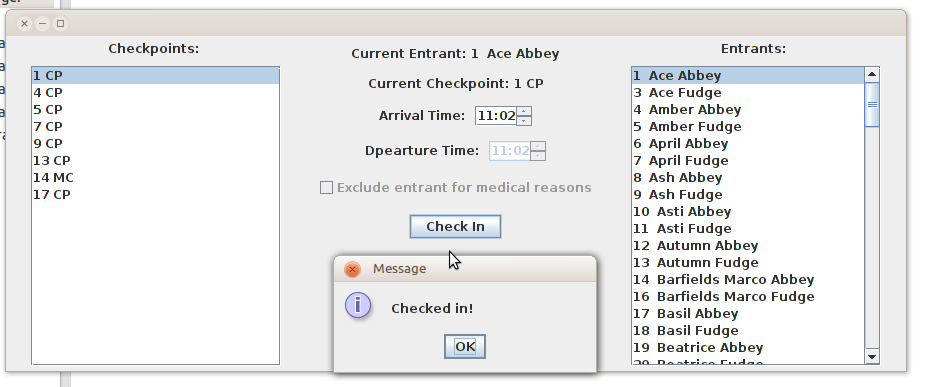
\includegraphics[width=1\textwidth]{img/GUI-test/valid-checkin.png}
\caption{Checking in a valid entrant at a valid time.}
\label{fig:valid-checkin}
\end{figure}

\subsubsection{Arriving at an Incorrect Node}
This example shows attempting to check in the same entrant as in the previous step to the same node directly after signing them in. This results in an a notice that the entrant will be excluded for going the wrong way on their course.

\begin{figure}[H]
\centering
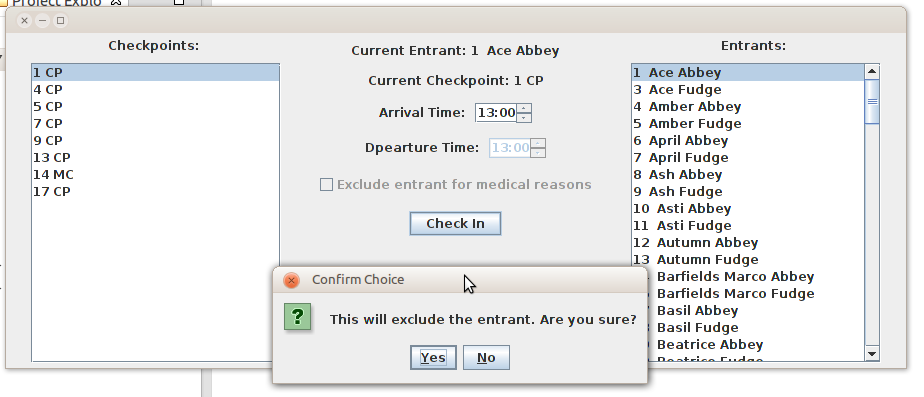
\includegraphics[width=1\textwidth]{img/GUI-test/invalid-checkin.png}
\caption{Checking in an entrant at an invalid node.}
\label{fig:invalid-checkin}
\end{figure}

\subsubsection{Arriving at Another Node at an Incorrect Time}
The next example shows checking in an entrant to a valid node (node 4) but at an invalid time (e.g. at a time before the last node they we're checked in at).

\begin{figure}[H]
\centering
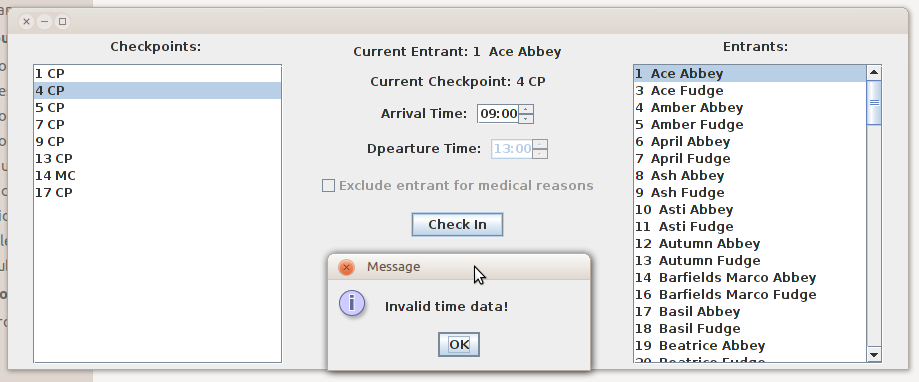
\includegraphics[width=1\textwidth]{img/GUI-test/invalid-time.png}
\caption{Checking in an entrant at a valid node but at an invalid time.}
\label{fig:invalid-time}
\end{figure}

\subsubsection{Checking into a Medical Checkpoint}
The following example shows checking in an entrant to a medical checkpoint. Notice how the relevant parts of the form are no longer greyed out when the medical checkpoint is selected.

\begin{figure}[H]
\centering
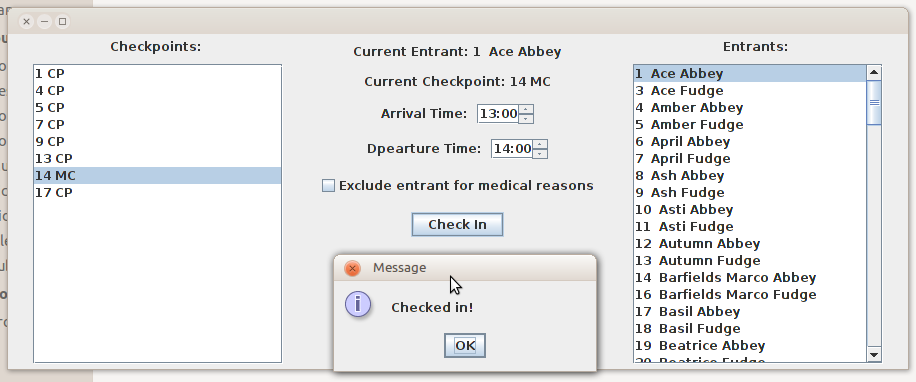
\includegraphics[width=1\textwidth]{img/GUI-test/mc-checkin.png}
\caption{Checking in an entrant at a medical checkpoint using valid times.}
\label{fig:mc-checkin}
\end{figure}

\subsubsection{Checking into a Medical Checkpoint with Incorrect Times}
This example shows attempting to check an entrant into a medical checkpoint with a departure time that is before the arrival time.

\begin{figure}[H]
\centering
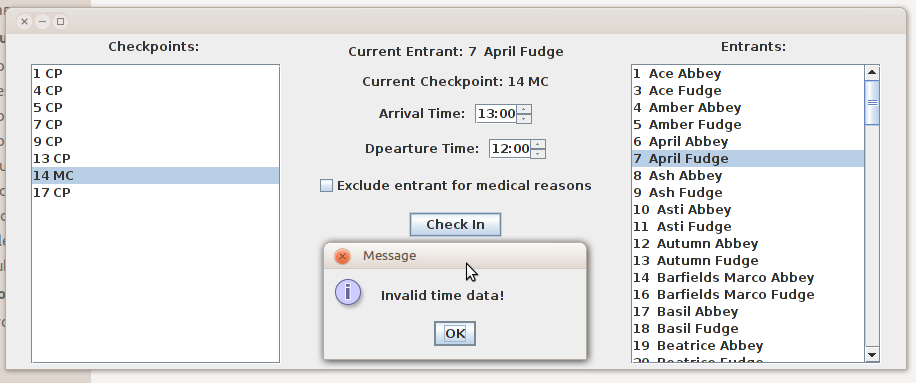
\includegraphics[width=1\textwidth]{img/GUI-test/mc-invalid-time.png}
\caption{Checking in an entrant at a medical checkpoint but with invalid arrival/departure times.}
\label{fig:mc-invalid-time}
\end{figure}

\subsubsection{Checking into a Medical Checkpoint and Excluding the Entrant}
The following example demonstrates the user interface when the user chooses to exclude an entrant for medical reasons from the event. Note that excluding an entrant at a checkpoint for going the wrong way but not for medical reasons works the same as at a regular checkpoint.

\begin{figure}[H]
\centering
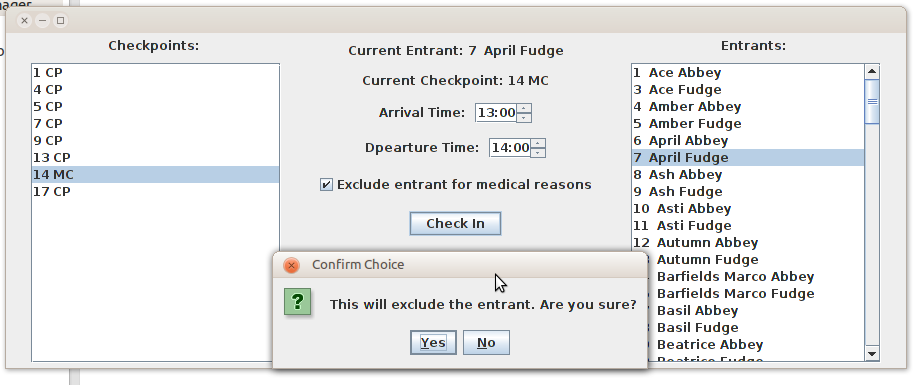
\includegraphics[width=1\textwidth]{img/GUI-test/mc-exclude.png}
\caption{Checking in an entrant at a medical checkpoint and excluding them at the same time.}
\label{fig:mc-exclude}
\end{figure}

\subsubsection{File Locking}
The final screen image shows what happens when the application tries to read the times file when another application has it open for writing. To demonstrate this functionality, I had to have one version of the application running from a jar file and another version running in debug mode with a breakpoint on line 290 of listing 26 to prevent the file lock from releasing the lock on the file.

\begin{figure}[H]
\centering
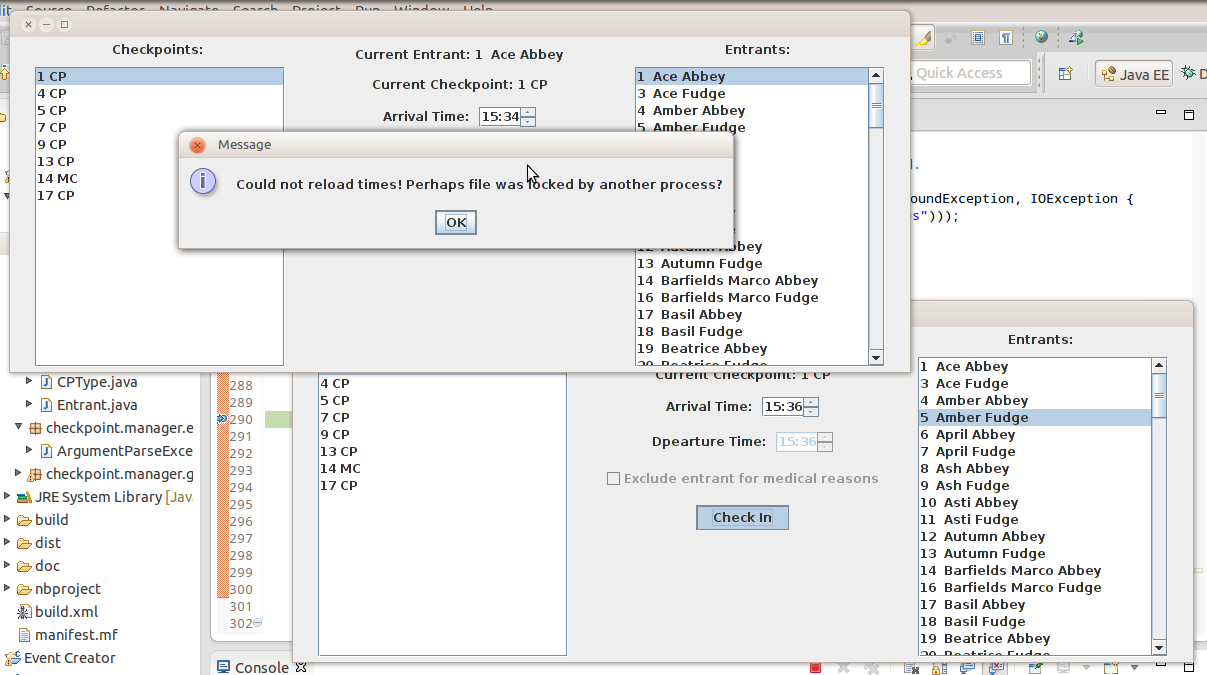
\includegraphics[width=0.6\textwidth]{img/GUI-test/file-lock.png}
\caption{Demonstrating file locking works by putting a break point in the lower right hand side application to prevent the lock from releasing.}
\label{fig:file-lock}
\end{figure}

\section{Event Manager Program Documentation}
This section provides the documentation for the Event Manager program, written in C, including build logs and example output.

\subsection{Compilation Output}
Below is the full build log from the compilation of the Event Manager program.

\begin{center}
	\begin{lstlisting}[showstringspaces=false, caption={Build log of the C Event Manager Program}]
	
12:27:50 **** Build of configuration Debug for project Event Manager ****
make all 
Building file: ../fileio.c
Invoking: GCC C Compiler
gcc -O0 -g3 -Wall -c -fmessage-length=0 -MMD -MP -MF"fileio.d" -MT"fileio.d" -o "fileio.o" "../fileio.c"
Finished building: ../fileio.c
 
Building file: ../linked_list.c
Invoking: GCC C Compiler
gcc -O0 -g3 -Wall -c -fmessage-length=0 -MMD -MP -MF"linked_list.d" -MT"linked_list.d" -o "linked_list.o" "../linked_list.c"
Finished building: ../linked_list.c
 
Building file: ../main.c
Invoking: GCC C Compiler
gcc -O0 -g3 -Wall -c -fmessage-length=0 -MMD -MP -MF"main.d" -MT"main.d" -o "main.o" "../main.c"
Finished building: ../main.c
 
Building file: ../util.c
Invoking: GCC C Compiler
gcc -O0 -g3 -Wall -c -fmessage-length=0 -MMD -MP -MF"util.d" -MT"util.d" -o "util.o" "../util.c"
Finished building: ../util.c
 
Building target: Event Manager
Invoking: GCC C Linker
gcc  -o "Event Manager"  ./fileio.o ./linked_list.o ./main.o ./util.o   
Finished building target: Event Manager
 

12:27:50 Build Finished (took 415ms)
		
	\end{lstlisting}
\end{center}

\subsection{Example Run Output}
The following section shows the output generated from running the event manager program for each type of query a user can make with the system. This run was carried out using event one example files.

\begin{center}
	\begin{lstlisting}[showstringspaces=false, caption={Output of an example run of the C program}]
		|==============================================|
|--------------RUNNERS AND RIDERS--------------|
|----------------------------------------------|
|----------Event tracking application----------|
|==============================================|

Loading data files...
Enter location and name of event details file:
../event_1/name.txt
Enter location and name of the nodes file:
../event_1/nodes.txt
Enter location and name of the tracks file:
../event_1/tracks.txt
Enter location and name of the courses file:
../event_1/courses.txt
Enter location and name of the entrants file:
../entrants.txt
Error opening file:
../entrants.txt
Enter location and name of the entrants file:
../event_1/entrants.txt
Enter location and name of the log file:
../event_1/log.txt
Enter location and name of the times file:
../event_1/cp_times_1.txt
Enter an Option:
0  - Exit
1  - Event Details
2  - Query Competitor
3  - Check how many competitors not yet started
4  - Check how many competitors are out on courses
5  - Check how many competitors have finished
6  - Print table of results
7  - Print entrants excluded at medical checkpoints
8 - Print entrants excluded at regular checkpoints
1
Endurance Horse Race - Beginners Event
26th June 2012
Start Time: 07:30
Enter an Option:
0  - Exit
1  - Event Details
2  - Query Competitor
3  - Check how many competitors not yet started
4  - Check how many competitors are out on courses
5  - Check how many competitors have finished
6  - Print table of results
7  - Print entrants excluded at medical checkpoints
8 - Print entrants excluded at regular checkpoints
2
Enter id for the competitor:
1
COMPETITOR 1:
Name: Donald Duck
Status: Out on track.
Last recorded time: 08:46
Last checkpoint visited: 9
Track Reference No.: 11
Presumed on track between node 3 and node 9
Enter an Option:
0  - Exit
1  - Event Details
2  - Query Competitor
3  - Check how many competitors not yet started
4  - Check how many competitors are out on courses
5  - Check how many competitors have finished
6  - Print table of results
7  - Print entrants excluded at medical checkpoints
8 - Print entrants excluded at regular checkpoints
3
0 competitors have not yet started
Enter an Option:
0  - Exit
1  - Event Details
2  - Query Competitor
3  - Check how many competitors not yet started
4  - Check how many competitors are out on courses
5  - Check how many competitors have finished
6  - Print table of results
7  - Print entrants excluded at medical checkpoints
8 - Print entrants excluded at regular checkpoints
4
13 competitors are out on a course
Enter an Option:
0  - Exit
1  - Event Details
2  - Query Competitor
3  - Check how many competitors not yet started
4  - Check how many competitors are out on courses
5  - Check how many competitors have finished
6  - Print table of results
7  - Print entrants excluded at medical checkpoints
8 - Print entrants excluded at regular checkpoints
5
0 competitors have completed their course
Enter an Option:
0  - Exit
1  - Event Details
2  - Query Competitor
3  - Check how many competitors not yet started
4  - Check how many competitors are out on courses
5  - Check how many competitors have finished
6  - Print table of results
7  - Print entrants excluded at medical checkpoints
8 - Print entrants excluded at regular checkpoints
6
-----------------------------------------------------------------------------------------------------------------
|Competitor           |  Course  |     Status     |  Start Time |   End Time  |    MC Delay    |     Total      |
|---------------------------------------------------------------------------------------------------------------|
|Donald Duck          |    D     |ON TRACK        |    07:30    |     N/a     |       N/a      |       N/a      |
|Mickey Mouse         |    D     |ON TRACK        |    07:35    |     N/a     |       N/a      |       N/a      |
|Jemima Julieta Mouse |    E     |ON TRACK        |    07:39    |     N/a     |       N/a      |       N/a      |
|Minnie Duck          |    F     |ON TRACK        |    07:43    |     N/a     |       N/a      |       N/a      |
|Minnie Mouse         |    E     |ON TRACK        |    07:47    |     N/a     |       N/a      |       N/a      |
|Minnie Mouse Junior  |    E     |ON TRACK        |    07:51    |     N/a     |       N/a      |       N/a      |
|Deputy Doug          |    D     |ON TRACK        |    07:56    |     N/a     |       N/a      |       N/a      |
|Deputy Duck          |    D     |ON TRACK        |    08:01    |     N/a     |       N/a      |       N/a      |
|Bewick Swan          |    F     |ON TRACK        |    08:05    |     N/a     |       N/a      |       N/a      |
|Black Swan           |    F     |TIME CHECKPOINT |    08:10    |     N/a     |       N/a      |       N/a      |
|Albert Einstein      |    E     |ON TRACK        |    08:14    |     N/a     |       N/a      |       N/a      |
|Albert Mouse         |    D     |ON TRACK        |    08:18    |     N/a     |       N/a      |       N/a      |
|Donald Duck Senior   |    E     |ON TRACK        |    08:22    |     N/a     |       N/a      |       N/a      |
|Egbert Einstein      |    F     |ON TRACK        |    08:26    |     N/a     |       N/a      |       N/a      |
-----------------------------------------------------------------------------------------------------------------
Enter an Option:
0  - Exit
1  - Event Details
2  - Query Competitor
3  - Check how many competitors not yet started
4  - Check how many competitors are out on courses
5  - Check how many competitors have finished
6  - Print table of results
7  - Print entrants excluded at medical checkpoints
8 - Print entrants excluded at regular checkpoints
7
Competitors Excluded from Medical Checkpoints
------------------------------------------
|Competitor           |  Node  |  Time   |
|----------------------------------------|
------------------------------------------
Enter an Option:
0  - Exit
1  - Event Details
2  - Query Competitor
3  - Check how many competitors not yet started
4  - Check how many competitors are out on courses
5  - Check how many competitors have finished
6  - Print table of results
7  - Print entrants excluded at medical checkpoints
8 - Print entrants excluded at regular checkpoints
8
Competitors Excluded from Regular Checkpoints
------------------------------------------
|Competitor           |  Node  |  Time   |
|----------------------------------------|
------------------------------------------
Enter an Option:
0  - Exit
1  - Event Details
2  - Query Competitor
3  - Check how many competitors not yet started
4  - Check how many competitors are out on courses
5  - Check how many competitors have finished
6  - Print table of results
7  - Print entrants excluded at medical checkpoints
8 - Print entrants excluded at regular checkpoints
0
	\end{lstlisting}
\end{center}

\subsection{Example Run Results List}
This sections show a listing of the results table for an event, including a selection of competitors in a variety of states (e.g. excluded, completed, not started etc.)

\begin{center}
	\begin{lstlisting}[showstringspaces=false, label={lst:results-output}, caption={The results table. With competitors in various states}]
-----------------------------------------------------------------------------------------------------------------
|Competitor           |  Course  |     Status     |  Start Time |   End Time  |    MC Delay    |     Total      |
|---------------------------------------------------------------------------------------------------------------|
|Donald Duck          |    D     |COMPLETED       |    15:32    |    19:32    |  00hrs 00mins  |  04hrs 00mins  |
|Mickey Mouse         |    D     |NOT STARTED     |    00:00    |     N/a     |       N/a      |       N/a      |
|Jemima Julieta Mouse |    E     |COMPLETED       |    15:35    |    18:35    |  00hrs 00mins  |  03hrs 00mins  |
|Minnie Duck          |    F     |COMPLETED       |    15:30    |    18:30    |  00hrs 00mins  |  03hrs 00mins  |
|Minnie Mouse         |    E     |EXCLUDED IR     |    00:00    |     N/a     |       N/a      |       N/a      |
|Minnie Mouse Junior  |    E     |NOT STARTED     |    00:00    |     N/a     |       N/a      |       N/a      |
|Deputy Doug          |    D     |NOT STARTED     |    00:00    |     N/a     |       N/a      |       N/a      |
|Deputy Duck          |    D     |NOT STARTED     |    00:00    |     N/a     |       N/a      |       N/a      |
|Bewick Swan          |    F     |NOT STARTED     |    00:00    |     N/a     |       N/a      |       N/a      |
|Black Swan           |    F     |NOT STARTED     |    00:00    |     N/a     |       N/a      |       N/a      |
|Albert Einstein      |    E     |NOT STARTED     |    00:00    |     N/a     |       N/a      |       N/a      |
|Albert Mouse         |    D     |NOT STARTED     |    00:00    |     N/a     |       N/a      |       N/a      |
|Donald Duck Senior   |    E     |EXCLUDED IR     |    00:00    |     N/a     |       N/a      |       N/a      |
|Egbert Einstein      |    F     |NOT STARTED     |    00:00    |     N/a     |       N/a      |       N/a      |
-----------------------------------------------------------------------------------------------------------------
	\end{lstlisting}
\end{center}

\subsection{Output Of Log File}
Below is the output of the log file after using the Checkpoint and Event manager applications to create the previous output.

\begin{center}
	\begin{lstlisting}[showstringspaces=false, caption={Output from the log file generated when creating the results shown in the listing \ref{lst:results-output}}]
	
16:30 CMP: Read the times file.
16:31 CMP: Read the times file.
16:31 CMP: Checked in entrant 4 @ node 1
16:31 CMP: Read the times file.
16:31 CMP: Checked in entrant 4 @ node 9
16:31 CMP: Read the times file.
16:31 CMP: Checked in entrant 4 @ node 13
16:31 CMP: Read the times file.
16:31 CMP: Read the times file.
16:31 CMP: Checked in entrant 4 @ node 1
16:32 CMP: Read the times file.
16:32 CMP: Checked in entrant 1 @ node 1
16:32 CMP: Read the times file.
16:32 CMP: Checked in entrant 1 @ node 4
16:32 CMP: Read the times file.
16:32 CMP: Read the times file.
16:32 CMP: Checked in entrant 1 @ node 5
16:32 CMP: Read the times file.
16:32 CMP: Checked in entrant 1 @ node 9
16:32 CMP: Read the times file.
16:32 CMP: Checked in entrant 1 @ node 1
16:34 CMP: Read the times file.
16:34 CMP: Checked in entrant 3 @ node 1
16:34 CMP: Read the times file.
16:34 CMP: Read the times file.
16:34 CMP: Checked in entrant 3 @ node 9
16:34 CMP: Read the times file.
16:34 CMP: Checked in entrant 3 @ node 13
16:35 CMP: Read the times file.
16:35 CMP: Checked in entrant 3 @ node 1
16:43 CMP: Read the times file.
16:43 CMP: Read the times file.
16:43 CMP: Checked in entrant 5 @ node 4
16:44 CMP: Read the times file.
16:44 CMP: Checked in entrant 13 @ node 4
16:45 EMP: Loaded the times file.
16:45 EMP: Viewed a list of results
16:45 EMP: Loaded the times file.

	\end{lstlisting}
\end{center}

\section{Outline of Programs}
This section of the document provides a brief outline of each of the three programs included as part of this project. This includes a discussion of the basic structure, design and operation of each application.

\subsection{Event Creation Program}
The event creation program is a command line based application written in C++. Its purpose is to create the event, courses and entrants file for each event. The design of the application allows the user to create multiple events at the same time, rather than having to make each event in serial. Because entrants need a course and a course needs an event, an event must be created before a course and a course must be created before an entrant. This includes the functionality to create different course and entrants associated with different events. Each event also expects a nodes file to be given when creating the event, allowing different events to work with different sets of allowed nodes. The user is also able to view an event by selecting the relevant option form the main menu.

Since lists of courses and entrants are associated with each event, I decided that the best approach would be to allow the user to create all the data about an event, then write it to file, rather than creating each of the files one at a time. When the user chooses the option to write an event, a new folder is created with the name of the event as the name of the folder. Inside the folder, the event, entrants and courses files are written.


\begin{figure}[H]
\centering
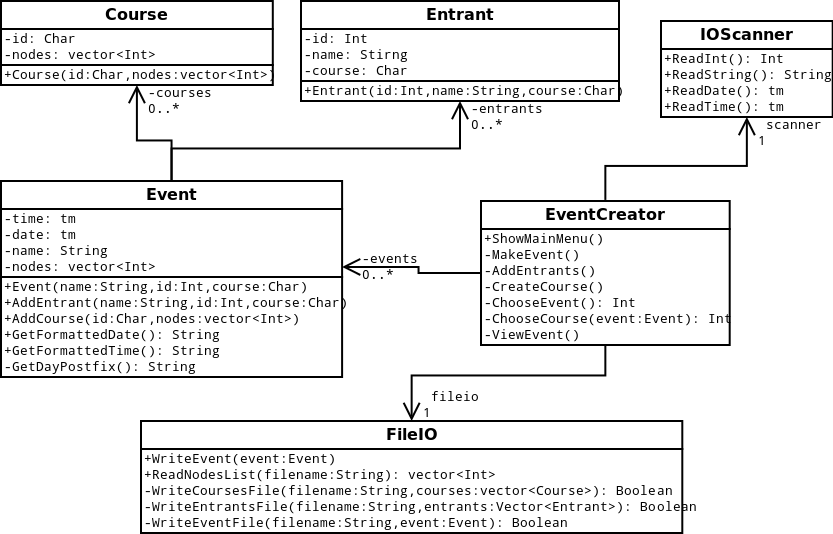
\includegraphics[width=0.6\textwidth]{diagrams/event_creator.png}
\caption{Class diagram of the Event Creator program. Getters/Setters not shown.}
\label{fig:GUI-image}
\end{figure}

\subsection{Checkpoint Manager Program}
The checkpoint manager program is written in Java and provides a Swing based GUI to allow the user to easily update entrants out in the field as the JVM allows the program to be executed on a variety of platforms. This program accepts the required files (entrants, courses, nodes, time and log files) as command line arguments using flags for each file. Help instructions are printed when no arguments or incorrect arguments are supplied. An example listing of arguments is supplied below:

\begin{center}
	\begin{lstlisting}[showstringspaces=false]
java -jar checkpoint_manager.jar -E ../../event_3/entrants.txt -C ../../event_3/courses.txt -K ../../event_3/nodes.txt
 -T ../../event_3/times.txt -L ../../event_3/log.txt

	\end{lstlisting}
\end{center}

The checkpoint manager program allows a race marshal to update the location of the entrants as they arrive at the various checkpoints on the course. Entrants are automatically excluded if checked into a checkpoint they should not of visited. The GUI also provides an option for marshals to excluded entrants based on failing a medical checkpoint. When an entrant is excluded, they are automatically removed from the list of available entrants. When an entrant is about to be excluded, the user is asked to confirm the operation, ensuring that they don't accidentally excluded a competitor.

\begin{figure}[H]
\centering
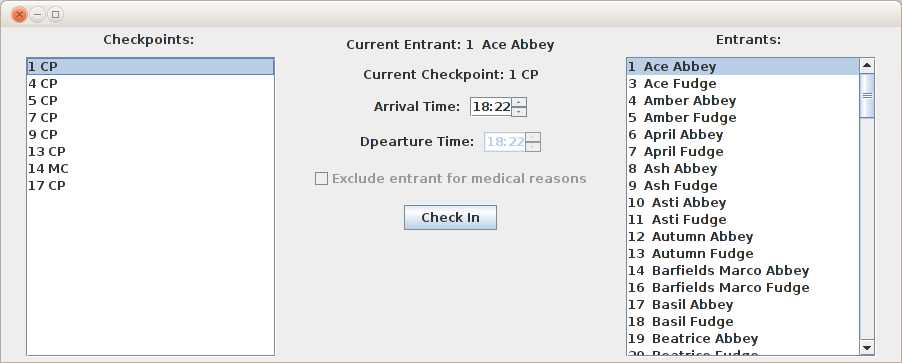
\includegraphics[width=0.5\textwidth]{img/GUI-screenshot.png}
\caption{Screen image of the Checkpoint manager GUI.}
\label{fig:GUI-image}
\end{figure}

\begin{figure}[H]
\centering
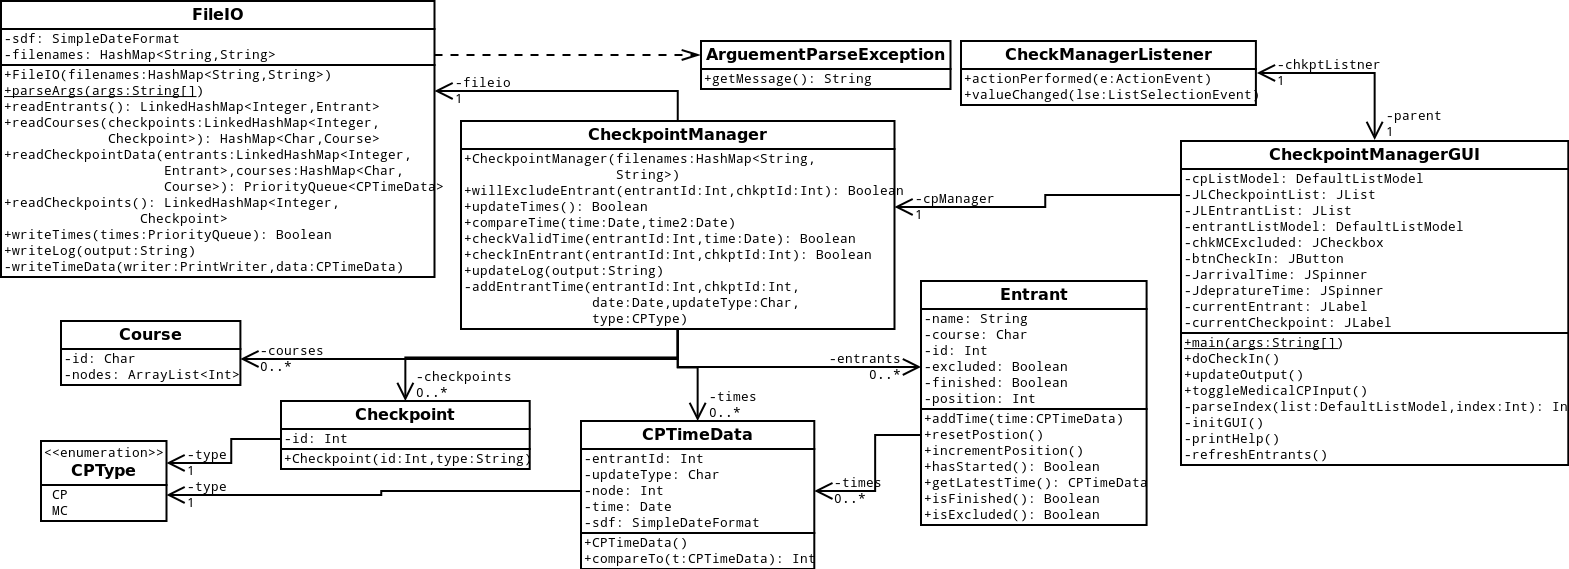
\includegraphics[width=1\textwidth]{diagrams/checkpoint_manager.png}
\caption{Class diagram of the Checkpoint Manager program. Getters/Setters not shown.}
\label{fig:GUI-image}
\end{figure}

The event manager program allows the user to input the time a competitor arrives and, in the case of medical checkpoints, departs. The program automatically checks that the arrival time is greater than the last time the entrant was checked in. In the case of medical checkpoints, it also checks that the arrival time is not greater than the departure time. Correct order of times is tracked using a priority queue.

\subsection{Event Manager Program}
The event manager program is written in C and handles checking the position and state of entrants as they progress through a course. This includes viewing a list of which entrants have been excluded, finished and are currently out on a track. It also gives the user the ability to query individual competitors and provides an estimate of what track/node they should/are on.

The event manager requires the loading of all the data files for an event. This is done by prompting the user at the start of the application and only needs to be done once. Like the event manager, the application locks the log and times file when reading to prevent multiple applications crashing during file processing.

\end{document}
